% -*- TeX-master: "../paper_notes.tex" -*-

\section{Antibunching  of  microwave  frequency  photons  observed  incorrelation
  measurements using linear detectors\label{sec:antibunching}}
\begin{enumerate}
\item Transmon qubit has energy of \iunit{8.0}{GHz}.
\item  Apply a  pulse with  phase $  \phi  $ and  duration $  \Omega  t =  \theta $  to get  a
  superposition:
 	
 	\[
          \ket{\psi} = \cos(\theta/2)\idown+\sin(\theta/2)\iup e^{i\phi}.
 	\]
      \item The transmon is placed near a resonator with \iunit{6.7}{GHz} and the
        two \red{\textbf{are  momenterally brought  into resonance by  applying a
            bias flux}}. According to  resonator-qubit interaction (Jaynes cummin
        Hamiltonian), the Hamiltonian for the system:
 	\[\begin{aligned}
            \mathcal{H}_{\text{middle}}
            & = \kbordermatrix{&\ket{\uparrow,N} & \ket{\downarrow,N+1}\\
              \bra{\uparrow,N} & \blue{\hbar\omega_r(N+\frac{1}{2}) + \hbar\Delta} & \red{g_0\sqrt{N+1}}\\
              \bra{\downarrow,N+1}  &  \red{g_0\sqrt{N+1}} &  \blue{\hbar\omega_r(N+\frac{1}{2})  -
                \hbar\Delta}}     \quad    \text{E}_{\pm}     =    \hbar\omega_r(N+\frac{1}{2})     \pm
            \frac{E_\text{coupled}}{2}
          \end{aligned}
 	\]
 	
 	\noindent so at resonance, we have unitary evolution:
 	\[
          \begin{aligned}
            U(t) & = \exp\big[-i(N+\frac{1}{2})\omega_r\mathbb{I} - i\frac{g_0\sqrt{N+1}}{\hbar}\sigma_x\big]\\
            & = e^{i\phi_\text{const}}\bigg[\cos(\frac{g_0\sqrt{N+1}}{\hbar}t)\mathbb{I}
            + i\sin(\frac{g_0\sqrt{N+1}}{\hbar}t)\sigma_x\bigg]
          \end{aligned}
 	\]
 	
 	\noindent so the state will evolve (top row is \iket{\uparrow, N}, bottom row is
        \iket{\downarrow, N+1})
 	\[
          U(t)    \ket{\psi}   =    e^{i\phi_\text{const}}\imatrix{\cos(\alpha   t)}{i\sin(\alpha
            t)}{i\sin(\alpha t)}{\cos(\alpha t)}\imatrixcol{\cos(\theta/2)}{e^{i\phi}\sin(\theta/2)}.
 	\]
 	
 	By choosing a time such that $ \alpha t  = \pi $ we get the state transferred to
        the cavity (resonator) which we can read out.
 	\[
          \begin{aligned}
            U(\pi/\alpha)\ket{\psi} = \cos(\theta/2)\iket{\uparrow, N} & + e^{i\phi}\sin(\theta/2)\iket{\downarrow, N+1} \ira (N = 0)\\
            \red{\ket{\text{outut    field}}}    &=    \red{\cos(\theta/2)\ket{0}    +
              \sin(\theta/2)e^{i\phi}\ket{1}}
          \end{aligned}
 	\]
 	
 	\red{Now  the cavity,  \iket{0}, \iket{1},  is storing  the state  of the
          qubit, so that we can read it out!}
      \end{enumerate}
      \iframe{The state that we are reading out from the cavity is
 	\begin{equation}\label{eqn:bunching_1}
          \ket{\psi} =  \imatrixcol{\cos(\theta/2)}{e^{i\phi}\sin(\theta/2)} \Rightarrow   				\rho = \frac{1}{2}\imatrix{1+{\cos(\theta)}{}}{e^{-i\phi}\sin(\theta)}{e^{i\phi}\sin(\theta)}{1-\cos(\theta)}
 	\end{equation}
        % \cos\left(\frac{\theta}{2}\right)\ket{0} +
        % e^{i\phi}\sin\left(\frac{\theta}{2}\right)\ket{1} =
      }

      \subsection{Measurements}
      \begin{enumerate}
      \item Field emitted from source is split \hfill $ E_{e,f}(t) $;
      \item Amplified\hfill $ E_{e,f}^{(+)}(t) $;
      \item Noise added \hfill $ E_{e,f}^{(+)}(t) + N_{e,f}(t) $;
      \item At this point, the `useful' signal' is mixed in with the freqeucny of
        the qubit - \red{we want to extract this envelope by hetrodyning}:
 	\begin{equation}\label{bunching1}
          E_{e,f}^{(+)}(t) + N_{e,f}(t) \ira \red{S_{e,f}(t)}e^{-i\omega t} \xrightarrow{hetrodyne} \red{S_{e,f}(t)}
 	\end{equation}
 	\begin{figure}[h]
          \begin{center}
            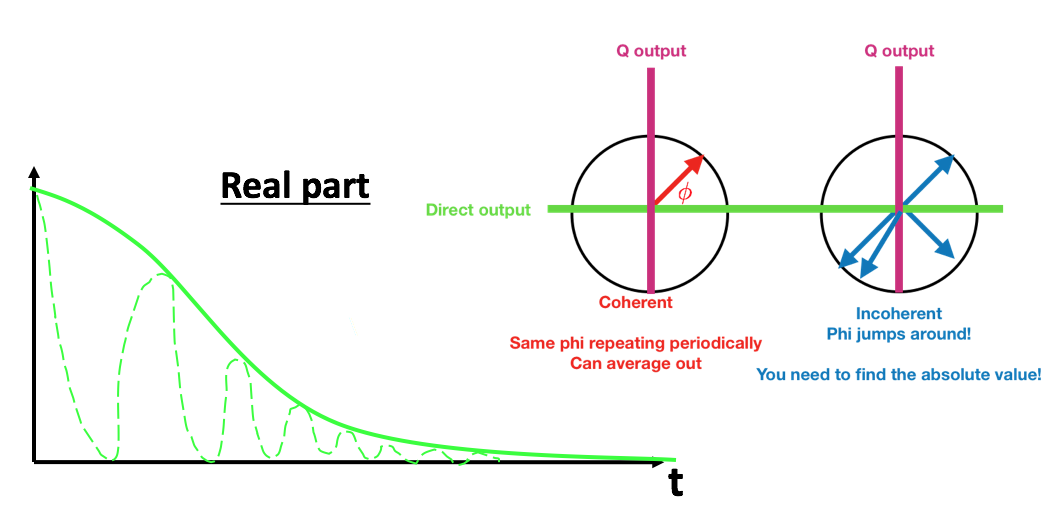
\includegraphics[height=5cm]{antibunch_1}
          \end{center}
          \caption{Once we have  extracted the envelope, its phsae  can either be
            fixed or jump around. \label{fig:bunching_1}}
 	\end{figure}
      \item  As  seen from  the  phase  image  above, \red{the  complex  envelope
          $ S_{e,f}(t) $} will have real and imaginary components (quadratures).
      \end{enumerate}
      So 4 combinations of outputs could be measured
      \begin{table}[h]
        \centering
        \begin{tabular}{|c|c|}
          \hline $ \re{S_e(t)} $ & $ \im{S_e(t)} $\\
          $ \re{S_f(t)} $ & $ \im{S_f(t)} $\\\hline
        \end{tabular}
      \end{table}
  
      % \begin{equation}\label{bunching2}
      %  	\text{Signal} \propto \iaverage{\hat{a}(t)}
      % \end{equation}
  
 \subsection{Direct amplitude measurements}
 \red{As will be shown in another paper}, when we measure one of the quadratures,
 in any one of the arms
  
  \begin{equation}\label{bunching3}
    \re{S(t)} \propto \iaverage{\hat{a}(t)}
  \end{equation}
  
  \noindent \red{\textbf{we will be probing  the expectation values of the cavity
      anhialation  operator.}}   The way  to  think  about  it  is, that  in  our
  \iket{0},\iket{1} basis

  \red{equation commented out}
  % \begin{equation}\label{eqn:bunching_4}
  %   \ialigned{
  %     \hat{a} & = \ketbra{0}{1}\\
  %     \iaverage{\hat{a}} & = \trace\lbrace\hat{a}\rho\rbrace\\
  %     \rho &= \frac{1}{2}\imatrix{1+{\cos(\theta)}{}}{e^{-i\phi}\sin(\theta)}{e^{i\phi}\sin(\theta)}{1-\cos(\theta)}
  %   } \ira \red{Re{S(t)} \propto \iaverage{\hat{a}} = \frac{1}{2}\cos(\phi)\sin(\theta)}.
  % \end{equation}
	
  \iframe{\textbf{So measuring the quadratue of the field} we are are probing
    \begin{equation}\label{bunching4}
      \re{S(t)} \propto \iaverage{\hat{a}} = \frac{1}{2}\cos(\phi)\sin(\theta)
    \end{equation}
    In the measurements  we see a direct  mapping of this pattern,  as we prepare
    different `amounts'  of the superposed  state (\red{corresponding to  the off
      diagonal elements of the density matrix}.)  \ipic{8cm}{anti_coherent}
    \begin{itemize}
    \item We  see the $  \sin(\theta) $ dependance.   Essentially, when we  rotate the
      state of the qubit, the phase $ \theta $ of the qubit changes.  At polar extrema
      ($  \theta =  0,  \pi$,  corresponding to  \iket{0},\iket{1})  there  is no  phase
      information \red{as there is no projection onto the equatorial plane!} This
      results  in no  quadrature  signal, as  every single  time  we perform  the
      measurement, the phase of the signal will jump randomly.
    \item The decay we see, is associated with the decay time of the cavity mode
      \begin{equation}\label{bunching5}
        T = \frac{Q}{\omega}.
      \end{equation} 
      \noindent  Once  the state  Eq.\eqref{eqn:bunching_1}  is  created, it  wil
      remain in the cavity  and slowly leak out. The `off  diagonal' terms of the
      state will dephase, and thus the signal will exponentially decay.
    \end{itemize}
  }
  \newpage \subsection{Full power measurements} In  the above section we measured
  the coherent part of the signal, by measuring direct voltage $ \re{S(t)} $.
  
  What if we now  measure power, by taking the absolute square  of the signal? We
  can use the input-output theory approach  to evaluate $ \iaverage{V^2(\omega)} $ and
  from it the total power $  1/Z\int\iaverage{V^2(\omega)}d\omega $ (done in the March summary
  report) to get
  
  \begin{equation}\label{eqn:dynamics1}
    \ialigned{\text{Total power} &= \hbar\omega\Gamma_1  \frac{1-{\isigmaz}_{}}{2}\\
      \text{Incoherent power} &= \hbar\omega\Gamma_1  \bigg[\frac{1-{\isigmaz}_{}}{2}-\isigmaplus\isigmaminus\bigg]
    }
  \end{equation}
  
  \noindent \iframe{And  getting the absolute  squared value of this  signal will
    this total power emitted from the qubit out for us
    \begin{equation}\label{eqn:bunching_2}
      \iaverage{S(t)^{*}S(t)} \propto \frac{1-\isigmaz}{2} = \frac{1 - \cos(\theta)}{2}.
    \end{equation}}

  \red{As we  shall see,  it very  much resembles what  is measured  during cross
    power measurements.}
  
  \subsection{Cross power - \textit{photon number in the line}}
  To evaluate cross  power, we mutliple out  the signals in the  two arms (taking
  complex conjugate because that is the  way the dot product between operators is
  defined.) \red{As shall be shown in another paper}
  
  \begin{equation}\label{bunching6}
    \iaverage{S_e^{*}(t) S_{f}(t)} \propto \iaverage{a^{\idagger}(t)a(t)}
  \end{equation}
  
  \noindent Now, operator $ a\idagger a = \hat{N} $ is the photon number operator
  which gives

  \begin{equation}\label{bunching7}
    \ialigned{
      &\text{Eq.~\eqref{eqn:bunching_1}}\qquad                \rho                 =
      \frac{1}{2}\imatrix{1+\cos(\theta)}{e^{-i\phi}\sin(\theta)}{e^{i\phi}\sin(\theta)}{1-\cos(\theta)} \\
      & \iaverage{\hat{O}} = \trace{a}\\%\hat{O}\rho
      & \hat{N} = 0\ketbra{0}{0} + 1\ketbra{1}{1}
    } \ira \iaverage{\hat{a}^{\dagger}\hat{a}} = \frac{1-\cos(\theta)}{2} = \sin^2(\theta/2).
  \end{equation}
  
  This is  the signal  observed in  the graphs  \iframe{ \textbf{The  cross power
      between the channels gives the photon number \iket{1} in the line}
    \begin{equation}\label{eqn:bunch_6}
      \iaverage{S_e^{*}(t) S_{f}(t)} \propto \iaverage{\hat{a}\idagger\hat{a}} = \sin^2(\theta/2)
    \end{equation}
    \ipic{8cm}{anti_incoherent}
    \begin{itemize}
    \item We see that $ \sin^2(\theta/2) $ dependance, where it depends on how excited
      we preapre the atom (peak is at $ \pi $);
    \item We see the same cavity decay time as for direct amplitude measurements.
    \end{itemize}
    \red{\underline{How in the world is this different from the signal we have in
        Eq.~\eqref{eqn:bunching_2}}? Well,  it is to  do with noise added  by the
      amplifiers.
  	
  	\begin{equation}\label{bunching8}
          \ialigned{
            \iaverage{S_e^{*}(t) S_{e}(t)} & \text{Noise of amplifier}, N_e(t)\\
            \iaverage{S_e^{*}(t) S_{f}(t)} & \text{Cross-noise of the noise in the two different amplifiers}, N_{e,f}(t)
          }
  	\end{equation}
  	\noindent   They   found    that   the   $   N_e(t)    \equiv   10.6\,$K   and
        $ N_{e,f}(t) \equiv \iunit{80}{mK}$, so there was much less noise being added!
      } }
    % \begin{figure}
    %   \begin{center}
    %     \input{testLatex}
    %   \end{center}
    % \end{figure}
 
 \subsection{Cross correlation}
 Now measures signals  with a time shift of  $ \tau $ and integrates  over the whole
 signal:
  
  \begin{equation}\label{eqn:bunching3}
    \Gamma^{(1)} = \int\iaverage{S_{e}^{*}(t)S_{f}(t+\tau)}dt - \Gamma^{(1)}_{ss} \propto \red{\int\iaverage{a\idagger(t)a(t+\tau)}dt},
  \end{equation}
  \noindent  where we  remove background  correlation $  \Gamma^{(1)}_{ss} $  which is
  measured between the photon pulses.
  
  \begin{itemize}
  \item  \iket{0}: There  are no  photons in  the ouput  line, so  no correlation
    signal;
  \item  \iket{1}: Photons  emitted at  different times  will have  absolutely NO
    coherence, as there is no projection  onto the equatorial plane. Reffering to
    Fig.~\ref{fig:bunching_1},  we say  that the  phase  is not  defined, and  so
    averaging over all events will result in a cancelation effect.
  \item  \isuperposition{+}: Each  time photons  will  be emitted  with the  same
    phase, and thus multipling
    \begin{equation}\label{bunching9}
      S_{e}^{*}(t)S_{f}(t+\tau),
    \end{equation}
    \noindent will accumulate a non zero value.
    \begin{itemize}
    \item   At    $   t   =   0    $,   we   have   the    cross   power   result
      $ \iaverage{a\idagger a} $, that  we had in Eq.~\eqref{eqn:bunch_6}, and we
      see this oscillation in $ \sin^2(\theta/2) $;
    \item  At $  t \neq  0$, both  $ S_e^{*}(t)  $ and  $ S_{f}(t+\tau)  $ will  have a
      repetitive  value,  both  in  phase  and amplitude.   This  means  that  in
      Eq.~\eqref{eqn:bunching3}
      \begin{equation}\label{}
        \int\iaverage{S_{e}^{*}(t)S_{f}(t+\tau)}dt \ra \int \iaverage{S_e^{*}(t)}\iaverage{S_{f}(t+\tau)}dt,
      \end{equation}
  	
      \noindent which means that from Eq.~\eqref{eqn:bunching_4}
  	
  	\begin{equation}\label{bunching10}
          \red{\re{S(t)} \propto \iaverage{\hat{a}} = \frac{1}{2}\cos(\phi)\sin(\theta)},
  	\end{equation}
  	
  	\noindent the signal will be $ \red{\propto \frac{1}{4}\sin^2(\theta)} $.
  	
      \end{itemize}
    \end{itemize}

    \ipicCaption{6cm}{bunch_2}{In the superposed state, the periodic photons will
      have the same defined phase, and thus will not cancel out, when we multiply
      out $ S_e(t)^{*}S_f(t+\tau) $ many times.\label{fig:bunch4}} \iframe{\red{Just
        to repeat -  the beam splitter does NOT split  the individual photon, but
        splits its  wavefunction into  arms $  e $  and $  f $.   The correlation
        function is probing the direct signal in the two arms}}.
	
 \subsection{The $ \Gamma^{(2)} $ function}
 Finally, the experiment was extended to measure
  
  \begin{equation}\label{bunching11}
    \Gamma^{(2)}(\tau) = \int \iaverage{S_{e}^{*}(t)S_{f}(t)S_{e}^{*}(t+\tau)S_{f}^{*}(t+\tau)}dt,
  \end{equation}
  
  \noindent known  as the  second order correlation  function. Essentially  it is
  probing the correlation between the power in the two arms of the system:
  
  \begin{itemize}
  \item At $ \tau = 0 $ we have $ \iabsSquared{S_{e}(t)}\iabsSquared{S_{f}(t)} $, so
    we are  measuring the average product  of the powers  in the two arms  of the
    interferometer. For a single photon source  the photon cannot split into both
    arms at the same time, so the average will be zero;
  \item  At $  \tau \neq  0$, we  can be  comparing the  powers shifted  by the  photon
    repitition frequency, so this will not be zero.
  	
    \ipicCaption{8cm}{bunching_4}{We  see a  dip at  $ \tau  = 0  $, since  a single
      photon cannot be in to arms at the same time - on average one will be zero,
      and    the    other    will    be    large.     We    also    notice    the
      $  \propto  \sin^4(\theta/2)$,   since  we  are  preparing  the   \iket{1}  states  as
      Fig.~\ref{fig:bunch4}.}   \red{How   is  this  different  from   the  above
      measurement, where we also measured the signal in both of the arms. Here we
      simply squared it. Then why does $ \tau = 0 $ suddenly vanish?}
  \end{itemize}
%%%%%%%%%%%%%%%%%%%%%%%%%%%%%%%%%%%%%%%%%%%%%%%%%

\newpage